\section{Exploration des données}
  Pour extraire les données correspondant à un certain seuil, nous avons utilisé la bibliothèque pandas permettant d'extraire des sous-ensembles de n-uplets dans un tableau en fonction de certains critères.
  Pour cela, nous avons écrit un code très simple [fig:\ref{fig:code_cut}] où R est le tableau de n-uplets et v est un dictionnaire contenant en clefs les modalités et en valeurs leur valeur seuil au-dessous de laquelle les n-uplets sont écartés.

\begin{figure}[H]
  \centering
  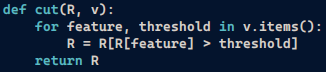
\includegraphics[scale=1]{images/code_cut.png}
  \caption{}
  \label{fig:code_cut}
\end{figure}

Pour enregistrer le JSON associé, nous avons choisi une nomenclature explicite qui correspond au dictionnaire de critères v, à savoir modalité1\_seuil1-modalité2\_seuil2-etc.json .
